\section{Softwarekonzept} \label{sec:softwarekonzept}

\subsection{Anforderung Software} \label{subsec:anforderungSoftware}

Die Software soll das Frequenzverhalten und die Einfügungsverluste von CM und DM des EMI-Filters simulieren können. Das Werkzeug soll insbesondere mit einer Empfindlichkeitsanalyse die Auswirkungen der parasitäreren Parameter auf die Einfügungsverluste des Filters darstellen. Die parasitären Filterparameter können in einem Bereich von ± 30\% variiert werden. Der Filter wird mit Hilfe von CM- und DM äquivalenten Schaltungsmodelle berechnet. Um die Auswirkungen der Parametervariation besser sichtbar zu machen, wird der Frequenzbereich des Filters in 3 Sektoren aufgeteilt: 0 kHz bis 500 kHz, 500 kHz bis 5 MHz und 5 MHz bis 30 MHz. 

Die folgende Konzeptbeschreibung der Software bezieht sich auf die maximal anzustrebende Lösung, dass heisst mit allen Wunschzielen inkludiert. Die Software wird so strukturiert, dass wenn diese Lösung nicht erreicht wird, die Software gut zur  maximal anzustrebende Lösung erweiterbar ist.

\subsection{GUI} \label{subsec:GUI}

Die GUI wird in 5 Teilbereiche aufgeteilt: Menu, Filtertabelle, CM/DM Plot, Buttonfenster und Eingabefenster. In der Abbildung \ref{fig:GUI} \nameref{fig:GUI} ist die Benutzerfläche des Programms dargestellt.

\begin{figure}[H]
	\centering
	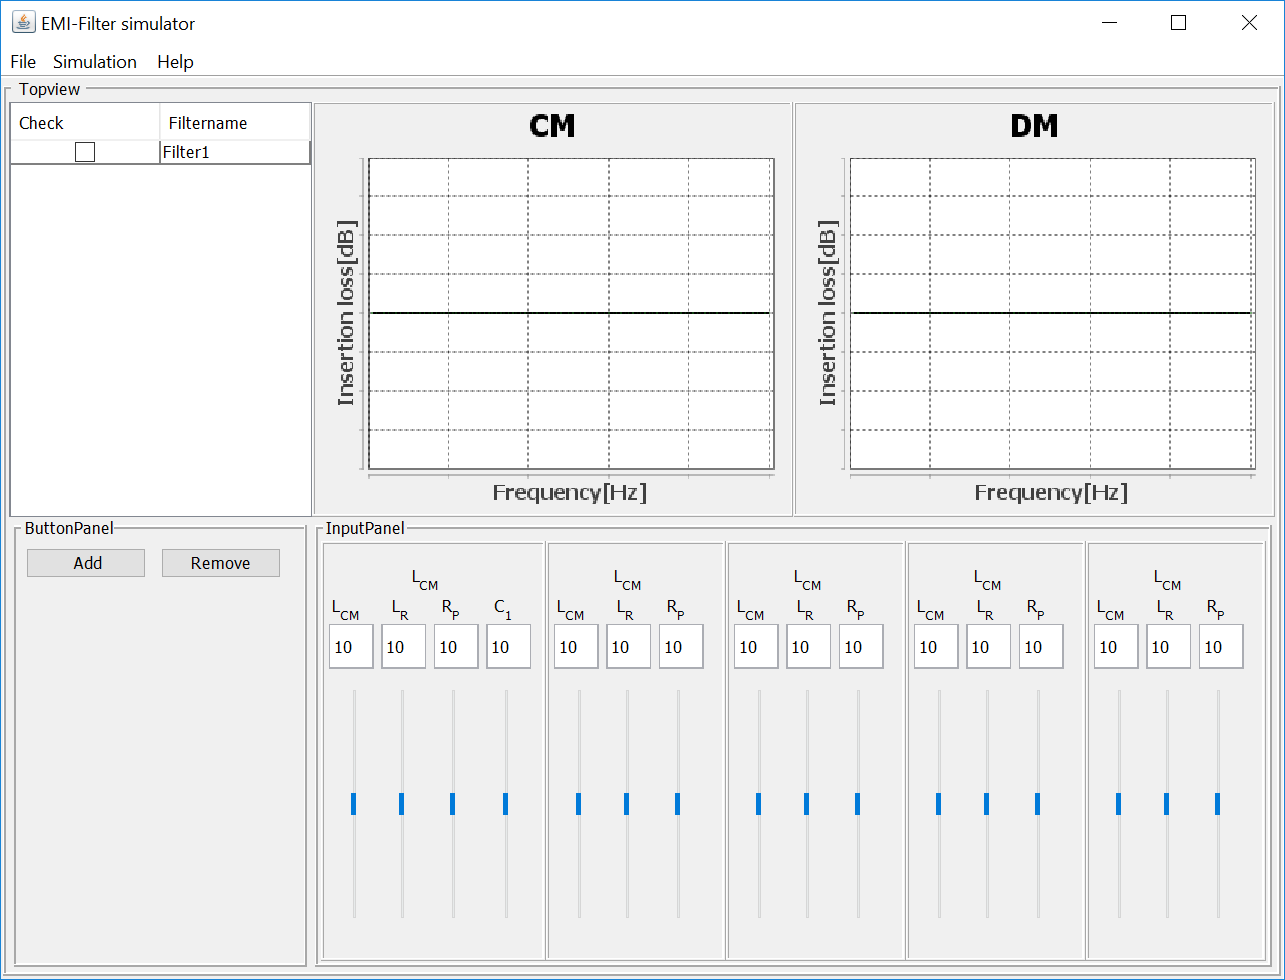
\includegraphics[width=10cm]{GUI.png}
	\caption{GUI}
	\label{fig:GUI}
\end{figure}

\newpage

\subsubsection{Menu} \label{subsubsec:menu}

Im Menu können verschiedene Optionen ausgewählt werden. Diese sind ebenfalls alle mit einem Shortcut aufrufbar.
\bigskip

\paragraph{File} \label{para:file}
Im Menupunkt "File" können Filterprofile gespeichert und geladen werden. Bei beiden Optionen wird der Explorer geöffnet um die .txt Datei im gewählten Verzeichnis abzulegen oder zu holen. In der Option Exit kann das Programm geschlossen werden. Dieser Menupunkt ist in der Abbildung \ref{fig:GUIFile} \nameref{fig:GUIFile} dargestellt.

\begin{figure}[H]
	\centering
	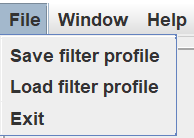
\includegraphics[width=4cm]{GUIFile.png}
	\caption{Menuoption File}
	\label{fig:GUIFile}
\end{figure}

\bigskip

\paragraph{Simulation} \label{para:simulation}
Im Menupunkt \"Simulation" kann die Simulationsart Monte Carlo ausgewählt werden. Es öffnet sich ein neues Fenster in dem der Parameter, die Toleranz und die Anzahl Messungen eingestellt werden kann. Dieser Menupunkt ist in der Abbildung \ref{fig:GUISimulation} dargestellt.

\begin{figure}[H]
	\centering
	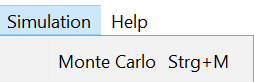
\includegraphics[width=4cm]{GUISimulation.png}
	\caption{Menuoption Simulation}
	\label{fig:GUISimulation}
\end{figure}

\bigskip

\paragraph{Help} \label{para:Help}
Im Menupunkt "Help" können die beiden CM- und DM äquivalenten Schaltungsmodelle, die zur Berechnung verwendet werden, in einem seperaten Fenster dargestellt werden. Dieser Menupunkt ist in der Abbildung \ref{fig:GUIHelp} \nameref{fig:GUIHelp} dargestellt.

\begin{figure}[H]
	\centering
	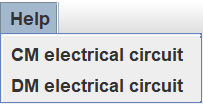
\includegraphics[width=4cm]{GUIHelp.png}
	\caption{Menuoption Help}
	\label{fig:GUIHelp}
\end{figure}

\newpage

\subsubsection{Filtertabelle} \label{subsubsec:filtertabelle}

In der Filtertabelle werden alle erstellte Filterprofile dargestellt und verwaltet. Mit einer Checkbox können einzelne Profile im Plot aus- bzw. eingeblendet werden. Zudem kann bei jedem Filterprofil einen Namen hinzugefügt werden. Die parasitären Filterparameter des ausgewählten Filterprofils werden in das Eingabefenster geladen und können dort verändert werden. Mit den Shortcuts Backspace and Delete können ausgewählte Profile gelöscht werden.

\subsubsection{CM/DM Plot} \label{subsubsec:CM_DMplot}

In den CM/DM Plots werden die Berechnungen logarithmisch visualisiert. Die Plots sind für die bessere Darstellung in 3 Frequenzbereiche aufgeteilt:0 kHz bis 500 kHz, 500 kHz bis 5 MHz und 5 MHz bis 30 MHz. Mit einem Rechtsklick auf den Plot können verschiedene Optionen ausgewählt werden. So können die Eigenschaften (Farbe, Darstellung, Schrift usw.) und der Zoom individuell eingestellt werden. Der Plot kann auch direkt in eine .png Datei abgespeichert oder gedruckt werden. Diese Optionen sind in der Abbildung \ref{fig:PlotSettings} \nameref{fig:PlotSettings} ersichtlich.

\begin{figure}[H]
	\centering
	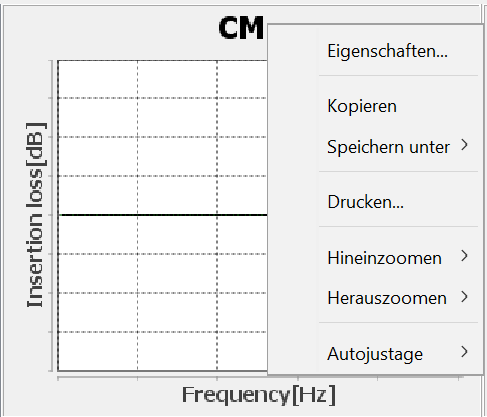
\includegraphics[width=4cm]{PlotSettings.png}
	\caption{Ploteinstellungen}
	\label{fig:PlotSettings}
\end{figure} 

\subsubsection{Buttonfenster} \label{subsubsec:buttonfenster}

Im Buttonfenster können Filterprofile in die Filtertabelle geladen oder entfernt werden. Mit dem Button Add werden die eingegebene parasitären Filterparameter in einem neuen Filterprofil gespeichert. Mit dem Button Remove wird das ausgewählte Filterprofil gelöscht. Der Button dient als alternative zu den Shortcuts.

\subsubsection{Eingabefenster} \label{subsubsec:eingabefenster}

Im Eingabebereich befinden sich die einzelnen parasitären Filterparameter. Es können Werte eingegeben und diese mit einer Toleranz von ± 30\% mit einem Schieberegler variiert werden. Die Werte werden direkt in die Filterprofile geladen, um eine Neuberechnung durchzuführen.

\newpage

\subsection{Softwarestruktur} \label{subsec:softwarestruktur}

Die Software wird mit dem Model-View-Controller Entwurfsmuster (MVC Design Pattern) \cite{MVCDesignPattern} strukturiert. Durch diese Strukturierung ist es weitgehende möglich die Daten und dessen graphischer Repräsentation zu trennen. Dies vereinfacht Wartungsarbeiten und die Wiederverwendbarkeit von Programmteile. Die Struktur ist in die drei Teilen Modell(engl. model), Präsentation(engl. view) und Steuerung(engl. controller) unterteilt

\subsubsection{Model} \label{subsubsec:model}

Im Model werden die Berechnungen ausgeführt. Die Daten werden vom Controller an die View übergeben. 

\subsubsection{View} \label{subsubsec:model}

In der View werden die Panel programmiert. Die Eingaben des Benutzers werden in der View erfasst und die Berechnungen des Models als plot angezeigt.

\subsubsection{Controller} \label{subsubsec:model}

Der Controller übermittelt die Daten der View and das Model indem er die entsprechende Methode aufruft. 

\subsubsection{Klassendiagramm} \label{subsubsec:model}

%TODO Klassendiagramm erstellen und einfügen


\subsection{Programmablauf} \label{subsec:programmablauf}

Beim Start des Programms werden die Panel initialisiert und die default Konfiguration hergestellt. Nun kann entweder ein neuer Filter erzeugt, oder ein bestehender Filter geladen werden. Ein bestehender Filter wird mittels "Menu / load Filter profile" aus einer Textdatei geladen. Ein neuer Filter wird mittels verändern der Schieberegler eingestellt und unter "Menu / save Filter" oder mittels "Ctrl + s" in ein .txt file gespeichert. Mittels button "Add" wird die Filtereinstellung temporär, bis zum schliessen des Programms gespeichert. An der linken Seite des Programms ist das Filterpanel. Darin werden alle eingestellten Filter aufgelistet und können mittels aktivieren der checkbox in verschiedenen Farben angezeigt werden. Der Einfluss eines bestimmten Parameters auf die Funktion kann mittels Monte Carlo Methode ermittelt werden. Dabei wird der Wert in kleinen Schritten verändert zum Beispiel von -10 bis + 10 Prozent und die Kurve für jeden Wert einmal abgebildet. So entstehen mehrere Kurven für die verschiedenen Parameter die man dann vergleichen kann.


\newpage
